\chapter{Estudo de caso}\label{cap:estudos_de_caso}

Dentro de um espaço conceitual da improvisação de códigos, selecionamos um exemplo específico, \emph{A Study in Keith} \cite{sorensen_keith_2009,sorensen_youtube_2014}, para ilustrar o intérprete concertista de \emph{jazz}, readequado para os propósitos do programador:

\begin{citacao}
\traducao{Para fundamentar a discussão em música, considere uma peça de \emph{jazz}, onde \emph{jazz} é um conceito e uma composição particular é uma instância de um conceito. O musicista, explorando os limites do \emph{jazz}, encontra então uma peça para além das regras usuais do \emph{jazz}. Através deste processo, os limites do gênero musical podem ser redefinidos em algum grau, ou se a peça está em um novo terreno particularmente fértil, um novo sub-gênero de \emph{jazz} emerge. Contudo uma peça de música que não quebra limites, de alguma forma pode ser considerada não-criativa \cite[p.~117]{McLean2011}.}{
To ground the discussion in music, consider a piece of jazz, where jazz is the concept and the particular composition is an instance of that concept. The musician, in exploring the boundaries of jazz, then finds a piece beyond the usual rules of jazz. Through this process, the boundaries of a music genre may be redefined to some degree, or if the piece is in particularly fertile new ground, a new sub-genre of jazz may emerge.  Indeed a piece of music which does not break boundaries in some way could be considered uncreative.}
\end{citacao}

São dois os registros audiovisuais principais, mas com duas descrições de um espaço conceitual \csf{E}{ask}, cuja semelhança é um referente opcional \pressingthree{R}{ask}{0}, ou os Concertos \emph{Sun Bear} \ver{sec:sunbear}:

\begin{citacao}
\traducao{\emph{A Study in Keith} é uma performance de programação ao vivo por Andrew Sorensen, inspirado nos concertos \emph{Sun Bear} de Keith Jarret. Toda a música que você ouve é gerada a partir do código do programa que é escrito e manipulado em \emph{tempo-real} durante a performance. O trabalho foi executado usando o ambiente de desenvolvimento $[$em linguagem$]$ Scheme $[$chamado$]$ Impromptu (\url{http://impŕomptu.moso.com.au}). Não é Keith, mas inspirado por Keith \cite{sorensen_youtube_2014}.
}
{
``A Study In Keith'' is a live programming performance by Andrew Sorensen inspired by Keith Jarrett's Sun Bear concerts. All of the music you hear is generated from the program code that is written and mani$[$p$]$ulated in real-time during the performance. The work was performed using the Impromptu Scheme software development environment (\url{http://impromptu.moso.com.au}). Not Keith, but inspired by Keith.
}
\end{citacao}

\citeonline{sorensen_youtube_2014} indica outros referentes, \pressingthree{R}{ask}{1} como o ambiente de programação \emph{Impromptu} e \pressingthree{R}{ask}{2} a linguagem de programação \emph{Scheme} \ver{sec:impromptu}:

\begin{citacao}
\traducao{\emph{A Study In Keith} é um trabalho para piano solo (NI's Akoustik Piano), inspirado nos concertos \emph{Sun Bear} de Keith Jarrett. \textbf{Note que não existe som para os dois primeiros 2 minutos da performance, enquanto estruturas iniciais são construídas}. Não é bem Keith, mas inspirado por Keith \cite{sorensen_keith_2009}}{"A Study In Keith" is a work for solo piano (NI's Akoustik Piano) by Andrew Sorensen inspired by Keith Jarrett's Sun Bear concerts. Note that there is no sound for the first 2 minutes of the performance while initial structures are built. Not quite Keith, but inspired by Keith.}
\end{citacao}


\section{Objetivo}\label{sec:objetivo}

Observação e análise de um comportamento criativo musical, de um improvisador-programador, que escreve uma programação-partitura, e realiza a manutenção de um pensamento musical tradicional. Mais especificamente, analisamos o contexto musical de uma simples sequência de blocos sonoros \pressingthree{K}{ask}{0}, gerada por uma função de interpretação $<<<$\csf{R}{ask}, \csf{T}{ask},\csf{E}{ask}$>>>$, cujo referente opcional direto, \pressingthree{R}{ask}{0}, são os Concertos \emph{Sun Bear} de Keith Jarret.

\section{Justificativa}

Parafraseamos \citeonline[p.~121]{McLean2011} ao afirmarmos que \traducao{Nosso estudo de caso é de alguma forma simplista e não é intenção ilustrar uma grande arte ou um grande código. Contudo delineia um processo criativo de classes, como efetuado pelo presente autor.}{Our case study is somewhat simplistic, and is not intended to illustrate either great art or great code. However it does trace a creative process of sorts, as carried out by the present author.}.


\section{Referentes Opcionais}\label{sec:sunbear}

A estratégia possui um referente opcional principal, \pressingthree{R}{ask}{0}, ou os Concertos \emph{Sun Bear}  de Keith Jarret \ver{sec:sunbearanal}, cuja análise possibilitou compreender simples estratégias harmônicas como regras de qualidade aplicadas em \emph{A Study in Keith}. Em seguida tratamos do timbre de piano utilizado \pressingthree{R}{ask}{1}, um \emph{plugin} VSTi \ver{sec:NI}, manipulado com um terceiro referente opcional, \pressingthree{R}{ask}{2}, ou o ambiente de programação musical chamado \emph{Impromptu} \ver{sec:impromptu}. 

\subsection{Concertos Sun Bear}\label{sec:sunbearanal}

Os concertos \emph{Sun Bear} são originalmente dez LPs  de improvisações de Keith Jarret no Japão, produzidos pela \emph{ECM Records}\footnote{http://www.ecmrecords.com/} entre 1976 e 1978. É o terceiro dos concertos de improvisação que incluem o \emph{Solo Concerts: Bremen/Lausanne} (1973) e \emph{The Köln Concert} (1975).

Foram realizados e gravados como sessões de improvisação contínua, variando entre 31 a 43 minutos cada. Para cada dia, duas sessões de improvisação, em cidades diferentes. Kyoto, 5 de novembro\footnote{Disponível em \url{https://www.youtube.com/watch?v=T2TfIQNxhjc}.}; Osaka, 8 de novembro\disponivelem{https://www.youtube.com/watch?v=FC4iZ1wMoU8}; Nagoya, 12 de novembro\footnote{\url{https://www.youtube.com/watch?v=3a7ezm3D1jA}.}. Tokyo, 14 de novembro\disponivelem{https://www.youtube.com/watch?v=ZH8VIjjhPQ4}; Sapporo, 18 de Novembro\disponivelem{https://www.youtube.com/watch?v=BqYBT_HoG4M}.


Um documento crítico impresso é mencionado na \emph{internet} como um antigo documento contendo notas discográficas \cite{rollingstone1985}. Seu acesso foi restrito durante a pesquisa, e não foi possível incluir alguma citação. Da mesma forma, documentos análiticos sobre a peça não foram encontrados em alguma base de dados. Existem algumas notas discográficas compiladas por uma comunidade de fãs e críticos musicais estadounidenses. Duas notas sugerem uma descrição da forma musical aplicada por Keith Jarret: \traducao{O tema de \emph{Kyoto Parte 1} é repetido por Keith Jarret no fim de \emph{Kyoto Parte 2}. Então podemos considerar o todo deste concerto como uma grande Suíte.}{The theme of Kyoto Part 1 is repeated By Kj at the end of Kyoto Part 2. So we can consider the whole of this concert as one big Suite}\cite[p.~129]{jarret_discography_2014}. 

\traduzcitacao{Revisto por Richard S. Ginnel\footnote{Disponível em \url{http://www.mcana.org/formembersatlarge.html}.}: $[$--$]$ Este pacote gigantesco -- um conjunto de dez LPs agora comprimidos em uma caixa robusta de seis $[$embalagens de$]$ CDs -- foi ridicularizado uma vez como uma última viagem de ego, provavelmente por muitos que não tomaram um tempo para ouvir tudo. (\ldots) Ainda assim, o milagre é como esta caixa é consistentemente muito boa. \textbf{Na abertura de Kyoto, a meditação direcionada para o \emph{gospel}} está em plena atuação, ao nível de suas melhores performances solo em Bremen e Koln,\textbf{e os concertos Osaka e Nagoya possuem citações de primeira linha, geralmente do tipo \emph{folk}}, mesmo profundas, idéias líricas
}{
Review by Richard S. Ginell: $[$--$]$ This gargantuan package -- a ten-LP set now compressed into a chunky six-CD box -- once was derided as the ultimate ego trip, probably by many who didn't take the time to hear it all. You have to go back to Art Tatum's solo records for Norman Granz in the '50s to find another large single outpouring of solo jazz piano like this, all of it improvised on the wing before five Japanese audiences in Kyoto, Osaka, Nagoya, Tokyo, and Sapporo. Yet the miracle is how consistently good much of this giant box is.  In the opening Kyoto concert, Jarrett's gospel-driven muse is in full play, up to the level of his peak solo performances in Bremen and Koln, and the Osaka and Nagoya concerts have pockets of first-rate, often folk-like, even profound, lyrical ideas.
}
{p.~130}
{jarret_discography_2014}

O \emph{gospel} e o \emph{folk} são citados como gêneros musicais inclusivos nesta suíte. Porém esta Suíte não possui pausas entre as partes (o improviso é contínuo, mas seccionado por transições). Uma transcrição do motivo gerador deste \emph{gospel} no concerto de Kyoto buscou encontrar referentes opcionais adicionais para \pressingtwo{R}{ask} (isto é, informações de harmonia e ritmo), mesmo com a afirmação anterior que nenhuma relação pode ser encontrada \ver{fig:Jarret_intro}. 

\begin{figure}[!h]
  \centering
  %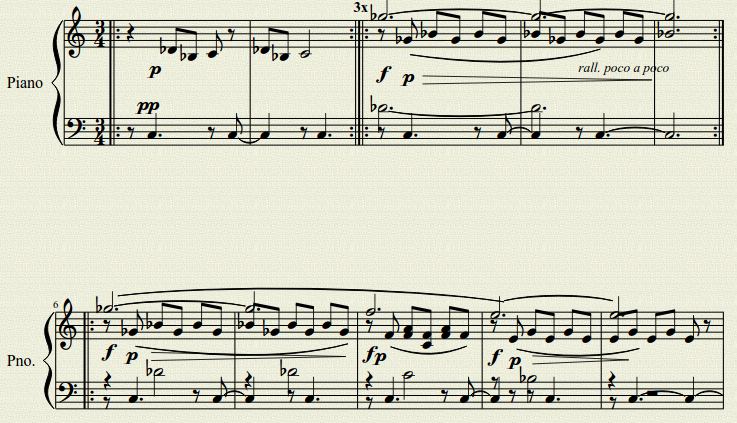
\includegraphics[scale=0.5]{imagens/Jarret_intro.png}
  {%
\parindent 0pt
\noindent
\ifx\preLilyPondExample \undefined
\else
  \expandafter\preLilyPondExample
\fi
\def\lilypondbook{}%
\input{b1/lily-fc418522-systems.tex}
\ifx\postLilyPondExample \undefined
\else
  \expandafter\postLilyPondExample
\fi
}
  \caption{Transcrição do motivo gerador do disco Kyoto, parte 1. \textbf{Fonte}: autor.}
  \label{fig:Jarret_intro}
\end{figure}

Uma sequência do blocos de eventos, \pressingthree{K}{KJ}{0} apresenta três blocos de eventos $[$\pressingthree{E}{KJ}{0}\ldots\pressingthree{E}{KJ}{2}$]$. Uma figura sincopada, que alterna uma nona menor, terça menor, segunda maior, e oitava, pode ser serparada como dois objetos \pressingthree{O}{KJ}{0} e \pressingthree{O}{KJ}{1}: um ostinato na mão esquerda que preenche todo \pressingthree{K}{ask}{0}, e uma sequência repetida seis vezes que alterna a terça menor e segunda maior. Nos compassos 3 a 5, ou o bloco de eventos \pressingthree{E}{KJ}{1}, aparecem mais dois objetos que formam uma relação harmônica de trítono com o baixo, um intervalo de quarta justa \pressingthree{O}{KJ}{2}, e um ostinato de terças maiores \pressingthree{O}{KJ}{3}. O acorde de Sol bemol Maior (transcrito assim para facilitar a leitura), é expandido nos compassos 6 a 10, ou \pressingthree{E}{KJ}{2}, gerando uma figura cromática proto-melódica, cuja trasncrição apresenta a seguinte cadência: Sol Bemol Maior, Fá Maior com sexta adicionada (ou Ré menor com sétima, em segunda inversão) e Dó Maior com sétima menor. Limitamo-nos a considerar a progressão do ponto de vista do \emph{blues}, se aproximando do \emph{gospel} através de uma exploração da subdominante e da cadência plagal. 

Tomando um \emph{blues} tradicional de 12 compassos, seguindo a fórmula $I^7~\Rightarrow~IV^7~\Rightarrow~I^7~\Rightarrow~I^7$ $\Rightarrow~IV^7~\Rightarrow~IV^7~\Rightarrow~I^7~\Rightarrow~I^7~\Rightarrow~V^7~\Rightarrow~IV^7~\Rightarrow~I^7~$, é possível separar os acordes 4 a 7 ($~I^7~\Rightarrow~IV^7~\Rightarrow~IV^7~\Rightarrow~I^7$). Em termos bodenianos \ver{sec:criatividade}, a partir de uma exploração da sequência completa, é possível transformar, por substituição de trítono, a subdominante da sequência (\emph{subV/IV}). Isto é, a substituição-padrão, $bV/V^7~\Rightarrow~I^7$, ou $bII^7~\Rightarrow~I^7$, passa a ser operacionalizada como uma anti-tônica (considerando a tônica desta região $I^7$)\footnote{\cfcite{soares_luteria_2015}.}.  O que pode ser notado como $(bV^7/V)/IV~\Rightarrow~IV^7$, ou $bII^7/IV~\Rightarrow~IV^7$  pode ser simplificado como $bV^7~\Rightarrow~IV^7$. No entanto, a transcrição de Jarret (considerando sua futura correção), suprime e transforma as sétimas, a caracterizar uma sonoridade de tensão progressiva com um baixo pedal. Uma tríade do quinto grau bemol, uma tétrade do quarto grau com sexta e quinta, e primeiro grau com sétima):  $bV~\Rightarrow~IV^6_5~\Rightarrow~I^7$.

Se a transcrição está correta ou não, este não é o maior problema. A questão principal que permanece é se Jarret realmente improvisou este início, ou preparou esta pequena célula, como estímulo para o restante do disco. Na página anterior, uma nota crítica lembra que este tema é recuperado no final da segunda parte do disco, o que reforça o argumento de uma estrutura pré-definida. Em \emph{Study in Keith} a mesma pergunta permanece: o código elaborado por \citeonline{sorensen_keith_2009}, e sua sonoridade resultante, é de fato uma improvisação de códigos, ou existe um agenciamento onde o improvisador delineia um objetivo inicial?

\subsection{NI-Akoustik Piano}\label{sec:NI}

O NI, é uma abreviação para \emph{Native Instruments}, uma empresa de tecnologias para áudio \footnote{Disponível em \url{http://www.native-instruments.com/en/company/}.}. O \emph{Akoustic Piano} é uma extensão (\emph{plugin}) VST, que emula diferentes pianos acústicos. Os instrumentos são gravados nota a nota por um complexo sistema de tomada de som, amostrados digitalmente, para então ser possível utilizar os registros como eventos MIDI\disponivelem{http://www.native-instruments.com/en/products/komplete/keys/definitive-piano-collection/}

Existe um objetivo artístico, de Sorensen e Swift, em capacitar a improvisação de códigos com o piano. Isso não quer dizer que é a máquina que improvisa, mas sim como um humano que improvisa com um mecanismo que gera detalhes dinâmicos, mas cuja estrutura é pré-definida. E \emph{A Study in Keith} pode ser observado como uma simulação para um trabalho posterior com o \emph{Disklavier} da Yamaha \ver{fig:disklavier}. Este último caso não é citado por \citeonline{sorensen_youtube_2014} e \citeonline{sorensen_keith_2009}, mas em \emph{Disklavier Sessions} \cite{sorensen_disklavier_2013}, este mesmo um outro referencial \pressingthree{R}{ask}{1}, é semelhante à atividade descrita em \emph{A Study in Keith}:

\begin{figure}[h]
  \centering
  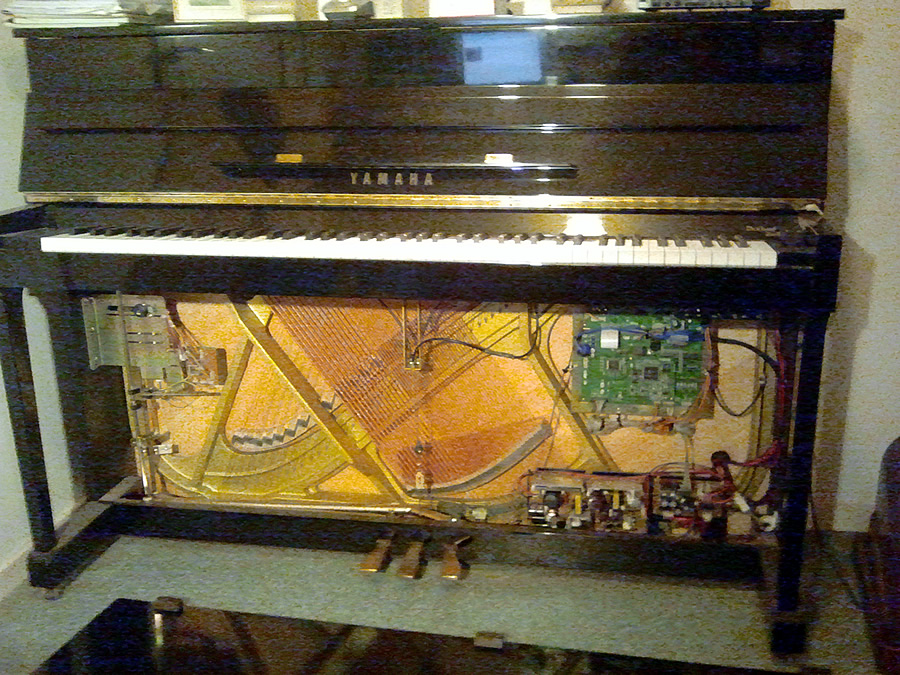
\includegraphics[scale=0.5]{imagens/disklavier.jpg}
  \caption{Piano Disklavier de armário, com a parte interna exposta para exibir a placa-mãe. \textbf{Fonte}: wikimedia.org}
  \label{fig:disklavier}
\end{figure}

\begin{citacao}
\traducao{Em \emph{Disklavier Sessions} os programas escritos em tempo-real por Ben e Andrew geram um fluxo de dados de notas que é enviado para ser executado em um piano disklavier mecanizado. Assim como as alturas das notas, toda a performance do piano deve ser codificada na informação gerada pelo programa e enviada para o piano disklavier.}{In the Disklavier Sessions the programs beign written in real-time by Ben and Andrew are generating a live stream of note data which is sent to a mechanized disklavier piano to be performed. As well the individual note pitches all of the piano performance must be encoded into the information being generated by the program and sent to disklavier piano}
\end{citacao}

Adiante daremos alguns detalhes de como Sorensen e Swift geram este fluxo de dados, que serão convertidos em ações do martelo do piano \ver{sec:eventos}. No momento, podemos dizer que são programados, em tempo-real, em um \emph{software}/Ambiente de programação nomeado como \emph{Impromptu}, cuja base de desenvolvimento é o \emph{Extempore}. 

\subsection{Ambiente e Linguagem: Impromptu}\label{sec:impromptu}

\begin{citacao}
\traducao{
Impromptu é uma linguagem e um ambiente de programação OSX\footnote{Sistema Operacional Mac OSX.} para compositores, artistas sonoros, VJ's e artistas gráficos  com um interesse em programação ao vivo ou interativa. Impromptu  é um ambiente de linguagem Scheme, um membro da família das linguages Lisp. Impromptu é usado por artistas-programadores em performances de \emph{livecoding} em torno do mundo.
}{
Impromptu is an OSX programming language and environment for composers, sound artists, VJ's and graphic artists with an interest in live or interactive programming. Impromptu is a Scheme language environment, a member of the Lisp family of languages. Impromptu is used by artist-programmers in livecoding performances around the globe.\emph{Disponível em \url{http://impromptu.moso.com.au/}}}
\end{citacao}

Segundo \citeonline[p.~823]{sorensen_impromptu_2010}, o Impromptu é um ambiente de programação ciberfísico, análogo à \emph{partitura} tradicional. O ambiente suporta a compilação de pequenos trechos de códigos executáveis em linguagem \emph{Scheme} (\csf{L}{ask}). Nos termos de \citeonline{magnusson_algorithms_2011}, os algoritmos codificados nesta linguagem são instrumento. Nos termos de \citeonline[p.~5]{fenerich_marulho_2014}, o código é uma programação-partitura:

\begin{citacao}
\traducao{Considere a analogia da partitura musical tradicional. A partitura provê uma especificação estática da intenção -- um programa de domínio estático. Musicistas, representam o domínio do processo, executam ações requeridas para realizar ouo reificar a partitura. Finalmente, as ações no domínio do processo resultam em ondas sonoroas que são percebidas por uma audiência humana como música. Este estágio final é o nosso domínio real de trabalho. Agora considere um domínio de programação dinâmica no qual o compositor concebe e descreve uma partitura em \emph{tempo-real}. Nós geralmente chamamos este tipo de composição de improvisação. \textbf{Na improvisação o(a) musicista é envolvido em um circuito-fechado retroalimentado que envolve premeditação, movendo para ação casual e finalmente para reação, refinamento e reflexão.}}{
Consider the analogy of a traditional musical score. The score provides a static specification of intention – a static program domain. Musicians, representing the process domain, perform the actions required to realise or reify the score. Finally, the actions in the process domain result in sound waves which are perceived by a human audience as music. This final stage is our real-world task domain. Now consider a dynamic program domain in which a composer conceives of and describes a musical score in real-time. We commonly call this type of composition improvisation. In it, the improvising musician is involved in a feedback loop involving forethought, moving to causal action and finally toreaction, refinement and reflection.}
\end{citacao}

Existe uma restrição quanto ao nicho de usuários do \emph{software}, com suporte para usuários de computadores Apple. Para lidar com outros sistemas (como por exemplo, sistemas operacionais Linux) e arquiteturas de processamento (32bit e 64 bit), o projeto foi liberado como código-aberto, com o nome \emph{Extempore}.

\subsection{Extempore}

O \emph{Extempore} possui um sistema humano-máquina reflexivo \ver{sec:grossi}. Um nome específico, para a atividade de programar, escutar o resultado, e recodificar, é simbolicamente chamado de \emph{programação ciberfísica}:

\begin{citacao}
\traducao{\emph{Extempore} é projetado para suportar um estilo de programação apelidado de $[$''$]$programação ciberfísica''.Programação ciberfísica suporta a noção de um programador humano operando como um agente ativo em uma rede de \emph{tempo-real} distribuída de sistemas ambientalmente conscientes} {Extempore is designed to support a style of programming dubbed 'cyberphysical' programming. Cyberphysical programming supports the notion of a human programmer operating as an active agent in a real-time distributed network of environmentally aware systems. \disponivelem{https://github.com/digego/extempore}. }
\end{citacao}

Entre suas características de interesse musical, incluem\disponivelem{http://benswift.me/2012/08/07/extempore-philosophy/}:

- Processamento de Sinais Digitais (DSP) \footnote{Sobre DSP, \cfcite{smith_dsp_2012}.} em  tempo-real;

- Sequenciamento de áudio de alto-nível, baseado em notas, como o disparo de sons baseado em parâmetros como altura, intensidade e duração. \disponivelem{http://benswift.me/2012/10/15/playing-an-instrument-part-i/}.;

A segunda característica será explorada neste capítulo como base técnica para o processo criativo em \emph{Study in Keith}

\subsection{Scheme}\label{sec:scheme}

Scheme é citado em diferentes fontes na \emph{internet} como uma definição de linguagem, ou dialeto, da linguagem Lisp (criado por John McCarthy em 1958), criado por Guy L. Steele e Gerald Jay Sussman em 1975. Uma das características da linguagem LISP é o tipo de representação de um código, ou seu padrão de notação, baseado em uma gramática generativa:

\begin{citacao}
\traducao{Um sistema chamado LISP (para Processador de LISta) foi desenvolvido para um computador IBM 704 pelo grupo de Inteligência Artificial no M.I.T. O sistema foi projetado para facilitar experimentos com um sistema proposto chamado ``Recebedor de conselhos'' $[$Advice Taker$]$, onde uma máquina pode ser instruída para lidar com sentenças declarativas, bem como imperativas, e poderia exibir um ``senso comum'' no desempenho de suas instruções. A proposta original para o \emph{Advice Taker} foi feita em novembro de 1958. O principal requerimento foi um sistema de programação para manipular expressões que representam sentenças formais, declarativas e imperativas, de modo que o sistema \emph{Advice Taker} pode fazer deduções. No curso do desenvolvimento, o sistema LISP passou por diversas simplificações e, eventualmente, se baseou em um esquema para representar funções recursivas parciais de certas classes de expressões simbólicas. Esta representação é independente do computador IBM 704, ou qualquer outro computador eletrônico, e agora parece útil expor o sistema, começando com a classe de expressões chamadas expressões-S e as chamadas funções-S \cite[seção 1]{mccarthy_recursive_1960}.}{A programming system called LISP (for LISt Processor) has been developed for the IBM 704 computer by the Artificial Intelligence group at M.I.T. The system was designed to facilitate experiments with a proposed system called the Advice Taker, whereby a machine could be instructed to handle declarative as well as imperative sentences and could exhibit ``common sense'' in carrying out its instructions. The original proposal [1] for the Advice Taker was made in November 1958. The main requirement was a programming system for manipulating expressions representing formalized declarative and imperative sentences so that the Advice Taker system could make deductions.In the course of its development the LISP system went through several stages of simplification and eventually came to be based on a scheme for representing the partial recursive functions of a certain class of symbolic expressions. This representation is independent of the IBM 704 computer, or of any other electronic computer, and it now seems expedient to expound the system by starting with the class of expressions called S-expressions and the functions called S-functions.}
\end{citacao}

A definição de funções-S foge do escopo de nossa pesquisa, mas ela pode ser compreendida de maneira intuitiva, a partir das expressões-S. \citeonline[seção~3]{mccarthy_recursive_1960} define expressões- S como ``átomos'' e listas de átomos, onde um átomo também pode ser uma lista de átomos. Existe uma classe de expressões simbólicas definida por parênteses. Dentro desta expressão simbólica são inseridos átomos (ver exemplo \ref{ex:s-expression}, \ref{ex:s-expression2} e \ref{ex:s-expression3}). 

%%%%%%%%%%%%%%%%%%%%%%%%%%%%%%%%%%%%%%%%%%%%%%%%%
\begin{example}{Expressão simbólica vazia}\label{ex:s-expression}
\begin{minted}[fontsize=\scriptsize]{cl}
( )
\end{minted}
\end{example}
%%%%%%%%%%%%%%%%%%%%%%%%%%%%%%%%%%%%%%%%%%%%%%%%%

Átomos, extraídos de sentenças abstratas, como listas de átomos:

%%%%%%%%%%%%%%%%%%%%%%%%%%%%%%%%%%%%%%%%%%%%%%%%%
\begin{example}{Expressão simbólica com átomos}\label{ex:s-expression2}
\begin{minted}[fontsize=\scriptsize]{cl}
;;A     -> 
( A )

;;AB    -> 
( A B )

;;ABA   ->
( A B A )

;;ABAC  ->
( A B A C )
( A B A C A )
\end{minted}
\end{example}
%%%%%%%%%%%%%%%%%%%%%%%%%%%%%%%%%%%%%%%%%%%%%%%%%

Átomos também podem ser eles mesmos outras expressões:

%%%%%%%%%%%%%%%%%%%%%%%%%%%%%%%%%%%%%%%%%%%%%%%%%
\begin{example}{Expressão simbólica com átomos}\label{ex:s-expression3}
\begin{minted}[fontsize=\scriptsize]{cl}
;;A = A
;;B = AB
;;C = BAB

;; ABA  -> 
( A ( A B ) A )
;; ABAC ->
( A ( A B ) A ( B A B ) )
( A ( A B ) A (( A B ) A ( A B )))

;;A = 1
;;B = +
;;C = 2

;; ABA  -> 
( 1 + 1 )   ;; = 2

;; ABAC -> 
( 1 + 1 2 ) ;; = 4
\end{minted}
\end{example}
%%%%%%%%%%%%%%%%%%%%%%%%%%%%%%%%%%%%%%%%%%%%%%%%%

A linguagem LISP implementa um tipo de notação chamada \emph{notação prefixada}, inventada por Jan Łukasiewicz em 1924, para simplificar a lógica proposicional ($P~\to~Q$). De fato, neste ponto, explicitamos uma característica da linguagem \csf{L}{ask}.Esta simplificação da notação pode, por exemplo, expressar uma proposição como  ``some uma unidade e uma unidade, logo teremos duas unidades'',  ou $1+1=2$, para uma operação indefinida, como ``some elementos, que neste caso, são dois unitários, logo duas unidades'', ou $+ 1 1$:

%%%%%%%%%%%%%%%%%%%%%%%%%%%%%%%%%%%%%%%%%%%%%%%%%
\begin{example}{Notação prefixada}
\begin{minted}[fontsize=\scriptsize]{cl}
;;A = 1
;;B = +
;;C = 2
;; ABA  -> BAA
( + 1 1 )  ;; = 2

;;ABAC -> BAAC -> 
( + 1 1 2 );; = 4
\end{minted}
\end{example}
%%%%%%%%%%%%%%%%%%%%%%%%%%%%%%%%%%%%%%%%%%%%%%%%%

Entre as diferenças do Lisp e Scheme, existe um vocabulário prédefinido para criação de sentenças, de forma que o significado do código possa ser legível, sem a necessidade de consideração de contextos. Para os propósitos deste trabalho definimos as variáveis e funções:

%%%%%%%%%%%%%%%%%%%%%%%%%%%%%%%%%%%%%%%%%%%%%%%%%
\begin{example}{Notação Scheme}
\begin{minted}[fontsize=\scriptsize]{cl}
;; define A = 1
(define A 1)

;; define B = 2
(define B 2)

;; divisao na forma (lambda argumentos operacao) 
(define divide            ;; define nome da funcao
        (lambda (a b)     ;; argumentos da funcao (calculo lambda)
                (/ a b))  ;; o que faz a funcao
)

;; execucao descritiva
(divide A B)
\end{minted}
\end{example}
%%%%%%%%%%%%%%%%%%%%%%%%%%%%%%%%%%%%%%%%%%%%%%%%%

Para os propósitos deste trabalho, será útil exemplificar musicalmente. \citeonline[p.~823-824]{sorensen_impromptu_2010} apresenta um pseudo-código musical, mais especificamente, direcionado para uma sonoridade de \emph{jazz} tonal. 

%%%%%%%%%%%%%%%%%%%%%%%%%%%%%%%%%%%%%%%%%%%%%%%%%
\begin{example}{Exemplo musical para o Scheme}

Este exemplo é semelhante com o primeiro algoritmo gerador de sonoridades tonais em \emph{A Study in Keith} \ver{sec:eventos}.

\begin{citacao}
\traducao{
\small{Dois performers se apresentam no palco. Um violinista, em pé e parado, com seu arco preparado. Outro senta-se atrás do brilho da tela do \emph{laptop}. Uma projeção da tela do \emph{laptop} é projetada acima do palco, e mostra uma página em branco, com um simples cursor piscando. O musicista-programador começa a digitar \ldots}
}{
Two performers are present on stage. One, a violinist, stands paused, bow at the ready. Another sits behind the glow of a laptop screen. A projection of the laptop screen is cast above the stage showing a blank page with a single blinking cursor. The laptop musician begins to type ...
}
\end{citacao}

\begin{minted}{cl}
( play-sound ( now ) synth c3 soft minute)
\end{minted}

\begin{citacao}
\traducao{
\small{\ldots a expressao é avaliada, e lampeja no retroprojetor para exibir a ação do executante. Um som etéreo sintetizado entra imediatamente no espaço e o violinista começa a improvisar em simpatia com a novidade da textura. O músico-programador, ouve o material temático fornecido pelo violinista e começa a delinear um processo generativo Markoviano para acompanhar o violino:}
}
{
\ldots the expression is evaluated and blinks on the overhead projection to display the performer’s action. An ethereal synthetic sound immediately enters the space and the violinist begins to improvise in sympathy with the newly evolving synthetic texture. The laptop performer, listens to the thematic material provided by the violinist and begins to outline a generative Markov process to accompany the violin ...
}
\end{citacao}


\begin{minted}[fontsize=\scriptsize]{cl}
( define chords
  ( lambda ( beat chord duration )
    ( for-each ( lambda ( pitch )
                   ( play synthj pitch soft duration ))
               chord )
    ( schedule (* metro * ( + beat duration )) chords
               (+ beat duration )
               ( random ( assoc chord (( Cmin7 Dmin7 )
                                       ( Dmin7 Cmin7 ))))
               duration )))

( chords (* metro * get-beat 4) Cmin7 4)
\end{minted}
%%%%%%%%%%%%%%%%%%%%%%%%%%%%%%%%%%%%%%%%%%%%%%%%%

\begin{citacao}
\traducao{\small{\ldots A função \emph{chords} é chamada no primeiro tempo de um nova barra de tempo, e uma simples progressão recursiva de acordes come a suportar a performance melódica do violino. A função \emph{chords} cria um laço temporal, gerando uma sequência interminável de acordes de quatro tempos. Depois de poucos momentos de reflexão, o musicista-programador começa a modificar a função \emph{chords} para suportar uma progressão de acordes mais variada, com uma razão aleatória $[$em função$]$ da recursão temporal\ldots}}
{\ldots the “chords” function is called on the first beat of a new common time bar and a simple recursive chord progression begins supporting the melodic performance of the violin. The chord function loops through time, creating an endless generative sequence of four beat chords. After a few moments of reflection the laptop performer begins to modify the “chords” function to support a more varied chord progression with a randomised rate of temporal recursion\ldots}
\end{citacao}

%%%%%%%%%%%%%%%%%%%%%%%%%%%%%%%%%%%%%%%%%%%%%%%%%
\begin{minted}[fontsize=\scriptsize]{cl}
( define chords
  ( lambda ( beat chord duration )
    ( for-each ( lambda ( pitch )
                   ( play dls (+ 60 pitch) soft duration ))
               chord )
    ( schedule (* metro * ( + beat duration )) chords
               (+ beat duration )
               ( random ( assoc chord (( Cmin7 Dmin7 Bbmaj )
                                       ( Bbmaj Cmin7 )
                                       ( Dmin7 Cmin7 )))
               ( random (3 6))))))

( chords (* metro * get-beat 4) Cmin7 4)
\end{minted}
\end{example}
%%%%%%%%%%%%%%%%%%%%%%%%%%%%%%%%%%%%%%%%%%%%%%%%%

Este pseudo-código será discutido, na próxima seção, como a estratégia transversal, \csf{T}{ask}. Propomos um particionamento do código para melhor compreensão:

%%%%%%%%%%%%%%%%%%%%%%%%%%%%%%%%%%%%%%%%%%%%%%%%%
\begin{example}{Nome da estratégia transversal}
\verb|chords| é o nome da estratégia.

\begin{minted}[fontsize=\scriptsize]{cl}
;; Definicao de acordes
( define chords
...
)
\end{minted}
\end{example}
%%%%%%%%%%%%%%%%%%%%%%%%%%%%%%%%%%%%%%%%%%%%%%%%%

\verb|chords| executado, como um impulso musical, com um único acorde com os seguintes parâmetros: momento de execução, grau e qualidade do acorde, duração do acorde:

\begin{example}{Estímulo inicial para a estratégia}
\begin{minted}[fontsize=\scriptsize]{cl}
; Execucao da funcao
( chords (* metro * get-beat 4) Cmin7 4)
\end{minted}
\end{example}


Adiante são definidas propriedades com termos do vocabulário da música tonal, ou, coloquialmente, batida (no sentido da posição de uma unidade de tempo em um pulso, \emph{tactus}), acorde (tríades, tétrades, formadas por relações de intervalos de terças maiores e menores), e duração (o quanto, em relação à unidade de tempo, este acorde irá durar):

%%%%%%%%%%%%%%%%%%%%%%%%%%%%%%%%%%%%%%%%%%%%%%%%%
\begin{example}{O que operacionaliza a estratégia}
\begin{minted}[fontsize=\scriptsize]{cl}
( ...
    ( lambda ( beat chord duration )
  ...
)    
\end{minted}
\end{example}
%%%%%%%%%%%%%%%%%%%%%%%%%%%%%%%%%%%%%%%%%%%%%%%%%%%

Existem duas estratégias internas na estratégia principal, cuja execução é realizada atavés de outras palavras-chaves. A palavra-chave \verb|for-each| realiza um laço iterativo para cada altura do acorde:

%%%%%%%%%%%%%%%%%%%%%%%%%%%%%%%%%%%%%%%%%%%%%%%%%%%%%%%%
\begin{example}{Laço iterativo para cada altura do acorde}
\begin{minted}[fontsize=\scriptsize]{cl}
;; Primeira estrategia interna 
;; Para cada acorde operacionalize cada altura
( for-each ( lambda ( pitch )
               ( play dls (+ 60 pitch) soft duration ))
           chord )
\end{minted}
\end{example}
%%%%%%%%%%%%%%%%%%%%%%%%%%%%%%%%%%%%%%%%%%%%%%%%%%%%%%%%%%

Para cada acorde \verb|chord|, é tocada uma nota (\verb|pitch|), com um centro em Dó 3 (MIDI 60), em piano (\verb|soft|) e uma duração padrão (\verb|duration|):

%%%%%%%%%%%%%%%%%%%%%%%%%%%%%%%%%
\begin{example}{Execução da nota}
\begin{minted}[fontsize=\scriptsize]{cl}
( play dls (+ 60 pitch) soft duration ))
\end{minted}
\end{example}
%%%%%%%%%%%%%%%%%%%%%%%%%%%%%%%%%%
A palavra-chave \verb|schedule| executa, recursivamente, um fluxo de acordes associados (\verb|random (assoc chord|), em resposta ao estímulo (\verb|( chords (* metro * get-beat 4) Cmin7 4)|). 

%%%%%%%%%%%%%%%%%%%%%%%%%%%%%%%%%%%%%%
\begin{example}{Fluxo de novos acordes}
\begin{minted}[fontsize=\scriptsize]{cl}
( schedule (* metro * ( + beat duration )) chords
               (+ beat duration )
               ( random ( assoc chord (( Cmin7 Dmin7 Bbmaj )
                                       ( Bbmaj Cmin7 )
                                       ( Dmin7 Cmin7 )))
               ( random (3 6))))
\end{minted}
\end{example}
%%%%%%%%%%%%%%%%%%%%%%%%%%%%%%%%%%%%%%%%

O momento de execução deste acorde depende da execução do acorde anterior

%%%%%%%%%%%%%%%%%%%%%%%%%%%%%%%%%%%%%%%%%%%%%%%%%%%%%%%
\begin{example}{Quando novos acordes serão computados}
\begin{minted}[fontsize=\scriptsize]{cl}
( schedule (* metro * ( + beat duration )) chords
                  ...
                  )
\end{minted}
\end{example}
%%%%%%%%%%%%%%%%%%%%%%%%%%%%%%%%%%%%%%%%%%%%%%%%%%%%%%%

Sendo que o acorde será executado logo em seguida que anterior terminar, com uma cadência harmônica escolhida dentre uma lista de cadências, com uma duração randômica entre três e seis unidades de tempo:

%%%%%%%%%%%%%%%%%%%%%%%%%%%%%%%%%%%%%%%%%%
\begin{example}{Propriedades de novos acordes}
\begin{minted}[fontsize=\scriptsize]{cl}
( schedule ... chords
               (+ beat duration )
               ( random ( ... ))
               ( random (3 6)))
\end{minted}
\end{example}
%%%%%%%%%%%%%%%%%%%%%%%%%%%%%%%%%%%%%%%%%%

A escolha de acordes é feita de maneira randômica, segundo uma lista de cadências predeterminados. Neste ponto, podemos indicar de maneira mais explícita uma regra de qualidade:

%%%%%%%%%%%%%%%%%%%%%%%%%%%%%%%%%%%%%%%%%%%%
\begin{example}{Propriedades de novos acordes}
\begin{minted}[fontsize=\scriptsize]{cl}
( random ( assoc chord (( Cmin7 Dmin7 Bbmaj )
                        ( Bbmaj Cmin7 )
                        ( Dmin7 Cmin7 )))
\end{minted}
\end{example}
%%%%%%%%%%%%%%%%%%%%%%%%%%%%%%%%%%%%%%%%%%%

Como definido pela função \verb|chords|, o acorde será tocado em um momento que depende do cronograma, cuja duração pode variar de 3 a 6 unidades de tempo. No caso, é prototipado um fluxo recursivo de acordes. Por exemplo, podemos restringir uma sequência de cadências-modelo com estruturas que se afastam da tônica, e as que voltam para a tônica. A maneira por qual podem ser acessadas, pode variar, e é interessante que o computador escolha randomicamente as progressões desejadas pelo improvisador programador \ver{fig:markov}. 

\begin{figure}
  \centering
  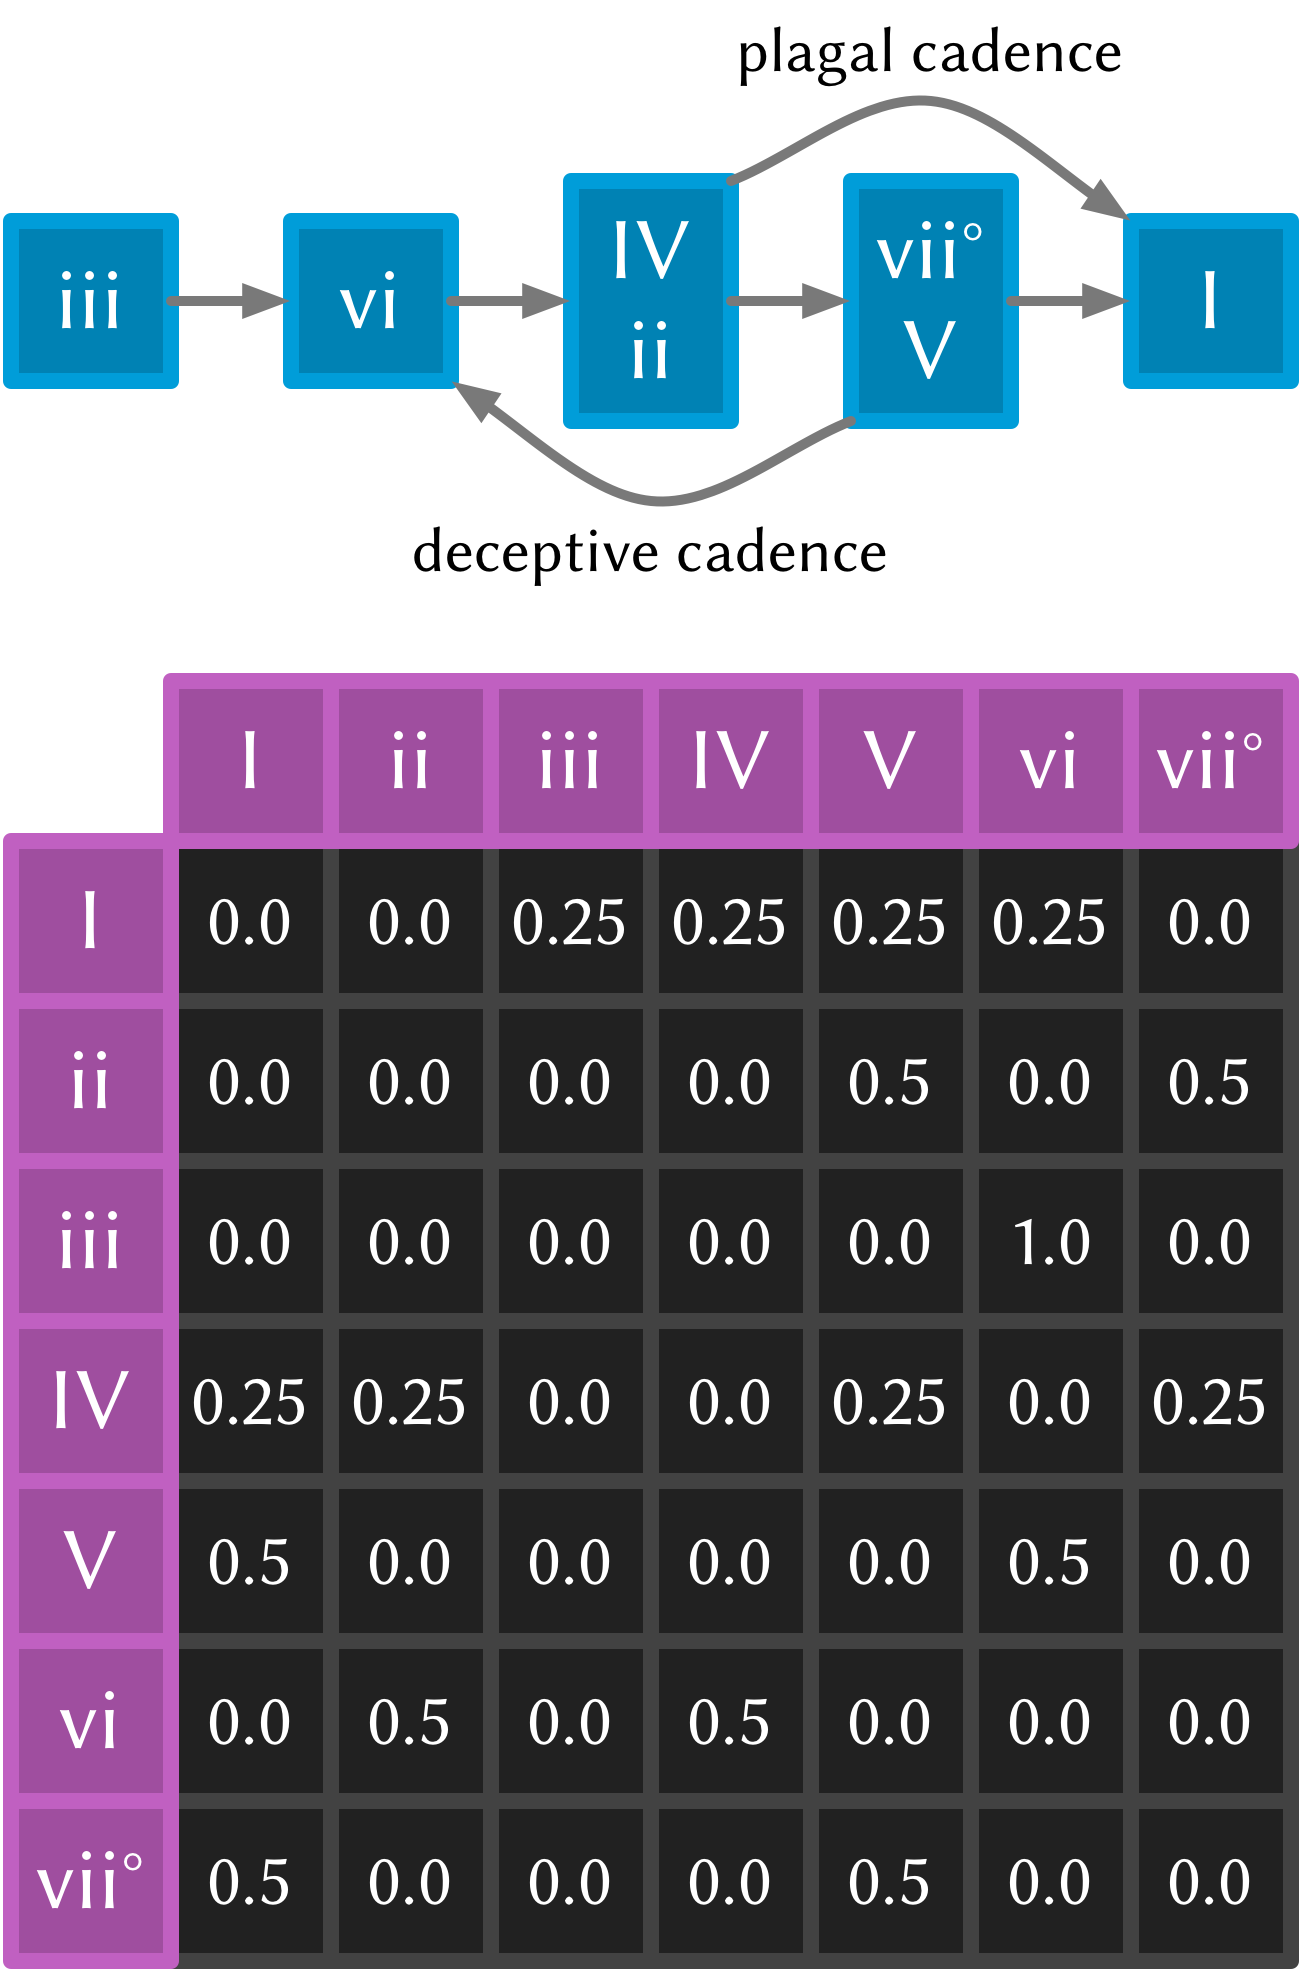
\includegraphics[scale=0.3]{imagens/markov.png}
  \caption{Distribuição, aproximada, de probabilidades de acontecimento com um conjunto de possíveis cadências tonais organizados como uma cadeia de Markov. \textbf{Fonte}: \citeonline{swift_playingII_2012}.}
   \label{fig:markov}
\end{figure}

No caso do bloco de código da explicação \citeonline[p.~823-824]{sorensen_impromptu_2010}, são utilizadas os seguintes movimentos harmônicos: $I^{7+}~\Rightarrow ii^{7}~\Rightarrow~IV^{7}/IV$, e $IV^{7}/IV~\Rightarrow~I^{7}$ e $ii^{7}~\Rightarrow~I^{7}$.

\subsection*{Discussão}

A partir de uma exploração destes referentes opcionais -- $[$\csf{R}{ask}{0},~\csf{R}{ask}{1},~\csf{R}{ask}{2}~$]$ -- foi possível classificar, além de uma linguagem \pressingthree{L}{ask}{0}, o algoritmo gerador da uma sonoridade tonal em \emph{Study in Keith}, ou \csf{T}{ask} \ver{sec:scheme}. Uma análise do algoritmo permite verificar algumas regras de qualidade \csf{E}{ask}. A interpretação $<<<$~\csf{R}{ask},~\csf{T}{ask},~\csf{E}{ask}~$>>>$ produziu uma sequência de blocos de eventos \pressingthree{K}{ask}{0} \ver{sec:eventos}. Outros blocos também são produzidos, porém nossa análise busca investigar o espaço conceitual que possibilitou os primeiros resultados em um ciclo de bricolagem.


\section{Blocos de Eventos}\label{sec:eventos}

No capítulo anterior, definimos o espaço conceitual, nos termos dos Quadros Conceituais de Sistemas Criativos, como uma aplicação do espaço conceitual da improvisação de códigos, e provavelmente, com um estilo de \emph{jazz}. Apresentamos algumas regras de validação em momentos anteriores, da improvisação de códigos \ver{sec:showusyourscreens}, e de um referencial opcional \ver{sec:sunbear}.

Seguiremos com configuração da estratégia transversal de Sorensen, como regra de detecção \csf{T}{ask}, que possui uma regra de qualidade \csf{E}{ask} \ver{sec:define_instr}. Este espaço conceitual gera uma sequência de blocos de eventos \pressingthree{K}{ask}{0}, muito semelhantes à neumas musicais básicos\footnote{\cfcite{gasperini_semiografia_1905}}, em um contraponto de primeira espécie que sofre uma primeira transformação \ver{sec:define_chords}. 

Uma nota sobre esta improvisação é feita pelo próprio Sorensen: nos primeiros dois minutos do vídeo (aproximadamente 1$'$53$''$). Existe um silêncio característico do momento em que os primeiros códigos são escritos. Este comportamento, do tempo de codificação, ao tempo de ação musical, é similar em outros dois vídeos, de Sorensen: \sorensen{An evening of livecoding at 53 Rusden Street}{https://vimeo.com/2433303}, \sorensen{Just for Fun}{https://vimeo.com/2433971}, \sorensen{A Study in Part}{https://vimeo.com/2434054}, \sorensen{Stained}{https://vimeo.com/2502546}, \sorensen{Transmissions in Sound}{Transmissions in Sound}, \sorensen{Antiphony}{https://vimeo.com/2503188},  \sorensen{Strange Places}{https://vimeo.com/2503257}, \sorensen{Orchestral}{https://vimeo.com/2579694}, \sorensen{UMDT}{https://vimeo.com/2579880}, \sorensen{Day of Triffords}{https://vimeo.com/2735394}, \sorensen{Face to Face}{https://vimeo.com/5690854}, \sorensen{BM\&E}{https://vimeo.com/7339135}, \sorensen{A Christimas Carol}{https://vimeo.com/8364077} \sorensen{Dancing Phalanges}{https://vimeo.com/8732631}, \sorensen{Livecoding Audio DSP}{https://vimeo.com/15585520}, \sorensen{Jazz Ensenble Study}{https://vimeo.com/15679078}, \sorensen{Variations on a Christmas Theme}{https://vimeo.com/18008372}. Esta característica também foi observada em uma outra performance \ver{sec:concerto}. Isso não quer dizer que o silêncio é um ator musical, com distância em relação a uma proposta apresentada anteriormente \ver{sec:coreografia}. 

\subsection{Definição do instrumento e do tempo}\label{sec:define_instr}

Seu início é um pequeno comentário que contem o nome do executante e seu email para contato (primeiros sete segundos), bem como a escrita de um código que inicializa o NI-Akoustik (até 0$'$43$''$, ver \autoref{fig:SIK_piano}). 

%%%%%%%%%%%%%%%%%%%%%%%%%%%%%%%%%%%%%%%%%
\begin{example}{Definição de instrumento}
  \centering 
Primeiros eventos musicais gerados a partir das primeiras estruturas válidas de código. \textbf{Fonte}: \cite{sorensen_youtube_2014}.
  \begin{minted}[fontsize=\footnotesize]{cl}
    ;;;;;;;;;;;;;;;;;;;;;;;;;;;;;;;;;;;;;;;;;;;;;;;;;
    ;; Andrew Sorensen andrew@moso.com.au
    (define piano (au:make-node "aumu" "NaDd" "-NI-"))
    (au:connect-node piano 0 *au:output-node* 0)
    (au:update-graph)

    (au:load-preset piano "/tmp/convert_grand.aupreset")
  \end{minted}
  \label{fig:SIK_piano}
\end{example}
%%%%%%%%%%%%%%%%%%%%%%%%%%%%%%%%%%%%%%%%%


Em \tempo{0}{52} Sorensen define um tempo base. Em seguida, Sorensen apaga o código para então iniciar definições de notas (\tempo{0}{54}).

%%%%%%%%%%%%%%%%%%%%%%%%%%%%%%%%%%%%%%%%%
\begin{example}{Definição de tempo}\label{ex:def_tempo}
  \centering
  Definição do tempo base. \textbf{Fonte}: \cite{sorensen_youtube_2014}.
  \begin{minted}[fontsize=\footnotesize]{cl}
    (define *metro* (make-metro 110))
  \end{minted}
  
\end{example}
%%%%%%%%%%%%%%%%%%%%%%%%%%%%%%%%%%%%%%%%%

\subsubsection{Definição de uma sequência de blocos}

Até \tempo{1}{07}, uma rotina auxiliar é definida como um laço iterativo. Porém não encontramos sua especificação no código-fonte do Extempore.

%%%%%%%%%%%%%%%%%%%%%%%%%%%%%%%%%%%%%%%%%
\begin{example}{Definição de uma função auxiliar}
  \begin{minted}[fontsize=\footnotesize]{cl}
    (pc:cb-for-each-p chords piano
                      (pc:make-chord 50 70 2 (pc:diatonic 0 '- degree))
                      dur)
  \end{minted}
\end{example}
%%%%%%%%%%%%%%%%%%%%%%%%%%%%%%%%%%%%%%%%%

Internamente, existe uma rotina que será o cerne de execução de uma nota, acompanhada de uma lista de 4 parâmetros (50, 70, 2):

%%%%%%%%%%%%%%%%%%%%%%%%%%%%%%%%%%%%%%%%%
\begin{example}{Definição de uma nota}\label{fig:SIK_acorde}
  \begin{minted}[fontsize=\footnotesize]{cl}
(pc:make-chord 50 70 2 (pc:diatonic 0 '- degree))
  \end{minted}
\end{example}
%%%%%%%%%%%%%%%%%%%%%%%%%%%%%%%%%%%%%%%%%

A abreviação \verb|pc| significa \emph{pitch class}, e a função \verb|pc:make-chord| significa que a função cria um acorde segundo parâmetros definidos no código-fonte do \emph{Extempore}\disponivelem{https://github.com/digego/extempore/blob/master/libs/core/pc_ivl.xtm}:

\begin{citacao}
\traducao{Cria uma lista do ``número'' $[$com$]$ alturas entre limites ``menor'' e ``maior'' do \emph{pc} dado. Uma divisão dos limites, pelo número de elementos requisitados, decompõem a seleção em extensões diferentes, do qual cada altura é selecionada. \emph{make-chord} tenta selecionar alturas para todos os graus do \emph{pc}. É possível, para  os elementos de um acorde resultarem em -1, se não existir nenhum \emph{pc} para a extensão dada. $[$É$]$ não-determinístico (i.e., resultados variam com o tempo). Argumento 1: limite menor (inclusivo). Argumento 2: Limite maior (exclusivo). Argumento 3: Número de alturas no acorde. Argumento 4: \emph{pitch class} \cite{swift_playingII_2012}.}{Creates a list of "number" pitches between "lower" and "upper" bounds from the given "pc". A division of the bounds by the number of elements requested breaks down the selection into equal ranges from which each pitch is selected.  \emph{make-chord} attempts to select pitches of all degrees of the pc.  It is possible for elements of the returned chord to be -1 if no possible pc is available for the given range. Non-deterministic (i.e. result can vary each time). arg1: lower bound (inclusive).  arg2: upper bound (exclusive). arg3: number of pitches in chord.  arg4: pitch class}
\end{citacao}

Este bloco de códigos cria uma díade, no âmbito de um Ré 2 (MIDI 50) e Si bemol 3 (MIDI 70), dentro de um campo harmônico diatônico (\verb|pc:diatonic|). Por sua vez, este último cria ``um acorde seguindo regras básicas de harmonia diatônca: baseado em uma raiz (0 para C, etc.), maior/menor (\verb|'-| ou \verb|'^|) e graus (i-vii)''\footnote{Tradução nossa de: \emph{(\ldots) a chord following basic diatonic harmony rules: based on root (0 for C etc.) maj/min ('- or '\^) and degree (i-vii)}.}. O resultado não é previsível, e depende de regras específicas de qualidade, que apresentaremos adiante, para classificar os \emph{pitch class} dentro de um grau de um campo harmônico.

\subsubsection {Definição de blocos}\label{sec:define_chords}

Em \tempo{1}{08}, a função \emph{chords} surge no fluxo audiovisual, sem nenhum processo de escrita. Este comportamento caracteriza a utilização de, ou uma cópia/cola de texto, ou de uma execução de um macro do editor de texto usado. Macros são pequenos programas no editor que auxiliam o processo de produção do código. De qualquer forma é importante salientar que o código é preparado \cite{sorensen_youtube_2014}.

%%%%%%%%%%%%%%%%%%%%%%%%%%%%%%%%%%%%%%%%%%%%%%%%
\begin{example}{Algoritmo que define os acordes}

O algoritmo apresenta apenas uma propriedade, tempo (\verb|time|).

\begin{minted}[fontsize=\footnotesize]{cl}
    (define chords
       (lambda (time)
          (for-each (lambda (p)
                       (play-note (*metro* time) piano p 80 (*metro* 'dur dur)))                                 
                    (pc:make-chord 50 70 2 (pc:diatonic 0 (quote -) degree)))
          (callback (*metro* (+ time (* .5 dur))) chords (+ time dur))))

    (chords (*metro* 'get-beat 4.0) 'i 3.0)
\end{minted}
\end{example}
%%%%%%%%%%%%%%%%%%%%%%%%%%%%%%%%%%%%%%%%%%%%%%%%

Primeiro é definida a estratégia transversal, \csf{T}{ask}, com um parâmetro, \verb|time|

%%%%%%%%%%%%%%%%%%%%%%%%%%%%%%%%%%%%%%%%%%%%%%%%
\begin{example}{Estratégia transveral}
\begin{minted}[fontsize=\footnotesize]{cl}
(define chords
   (lambda (time) ... ))
\end{minted}
\end{example}

Seguido de um ``impulso'', ou um estímulo sonoro:

%%%%%%%%%%%%%%%%%%%%%%%%%%%%%%%%%%%%%%%%%%%%%%%%
\begin{example}{Impulso, ou acorde inical}
\begin{minted}[fontsize=\footnotesize]{cl}
     (chords (*metro* 'get-beat 4.0) 'i 3.0)
\end{minted}
\end{example}
%%%%%%%%%%%%%%%%%%%%%%%%%%%%%%%%%%%%%%%%%%%%%%%%

Dentro de \csf{T}{ask}, é executado um laço iterativo, \verb|for-each|, para cada nota de uma díade.

%%%%%%%%%%%%%%%%%%%%%%%%%%%%%%%%%%%%%%%%%%%%%%%%
\begin{example}{Laço iterativo}\label{sec:iterativo}
\begin{minted}[fontsize=\footnotesize]{cl}
(for-each (lambda (p)
             (play-note (*metro* time) piano p 80 (*metro* 'dur dur)))                                 
          (pc:make-chord 50 70 2 (pc:diatonic 0 (quote -) degree)))
\end{minted}
\end{example}
%%%%%%%%%%%%%%%%%%%%%%%%%%%%%%%%%%%%%%%%%%%%%%%%

Cada nota é executada com uma altura \verb|p|, para cada díade definida em \verb|pc:make-chord|, em um momento definido por \verb|time| em relação ao pulso rítmico, com uma duração ainda a ser definida. 

%%%%%%%%%%%%%%%%%%%%%%%%%%%%%%%%%%%%%%%%%%%%%%%%
\begin{example}{Execução da nota}
\begin{minted}[fontsize=\footnotesize]{cl}
(play-note (*metro* time) piano p 80 (*metro* 'dur dur))
\end{minted}
\end{example}
%%%%%%%%%%%%%%%%%%%%%%%%%%%%%%%%%%%%%%%%%%%%%%%%

\verb|play-note| é definido com os seguintes argumentos, momento de execução ($time~\Rightarrow~(*metro* time)$), o instrumento tocado, ($instr~\Rightarrow~piano$), a altura ($pitch~\Rightarrow~p$), o volume ($vol~\Rightarrow~80$) e a duração do acorde ($dur~\Rightarrow~(*metro* 'dur dur)$)\disponivelem{https://github.com/digego/extempore/blob/5aec8b35c6b3058d1c66de7abf752dc667ab61e4/libs/core/instruments-scm.xtm}. 

\subsection{Primeira sonoridade tonal}\label{sec:1aSonoridade}

Este código inicial é então modificado, e finalizado em \tempo{1}{57}, momento em que é possível ouvir uma figura musical (uma classe de objeto \pressingthree{O}{ask}{0}), duas díades, um intervalo de quarta justa entre Sol 2 (MIDI 55) e Dó 3 (MIDI 60). entre Mi bemol 2 (MIDI 51) e Dó 3 (MIDI 60).

%%%%%%%%%%%%%%%%%%%%%%%%%%%%%%%%%%%%%%%%%%%%%%%%
\begin{example}{Estratégia transversal}
\begin{minted}[fontsize=\footnotesize]{cl}
    (define chords
       (lambda (time degree dur)
          (if (member degree '(i)) (set! dur 3.0))
          (for-each (lambda (p)
                       (play-note (*metro* time) piano p
                                  (+ 50 (* 20 (cos (* pi time))))
                                  (*metro* 'dur dur)))
                    (pc:make-chord 50 70 2 (pc:diatonic 0 (quote -) degree)))
          (callback (*metro*) (+ time (* .5 dur))) chords (+ time dur)
                    (random (assoc degree '((i vii)
                                            (vii i))))
                    dur))
    
     (chords (*metro* 'get-beat 4.0) 'i 3.0)
\end{minted}
\end{example}
%%%%%%%%%%%%%%%%%%%%%%%%%%%%%%%%%%%%%%%%%%%%%%%%

Duas transcrições desta primeira figura seguem uma estrutura literal do código, e uma perceptiva. Os primeiros eventos sonoros que ocorrem após o momento de silêncio foram transcritos antes da análise do código. Enquanto Sorensen define um tempo regular de 110 BPM  \ver{ex:def_tempo}, transcrevemos este trecho com um andamento entre 35--40 BPM \ver{fig:ask1}. É interessante notar que tais figuras simbolizam neumas, no caso, um \emph{bipunctum}, ou duas notas repetidas, na mão direita, e na mão esquerda um \emph{clivis}, ou um \traducao{acento agudo com um grave}{\cfcite[\emph{idem}]{gasperini_semiografia_1905}. Unione dell'accento acuto col grave}. No caso específico desta primeira figura, na mão direita, um \emph{bipunctum} , e na mão esquerda, uma \emph{clivis}.

\begin{figure}[!h]
  \centering
  \centering 
  \input{./ask1}
  \input{./ask2}
  \input{./gregorian}
  \caption{Transcrição literal e perceptiva do primeiro evento em \emph{A Study in Keith}. \textbf{Fonte}: autor.}
  \label{fig:ask1}
\end{figure}

 É importante notar que algumas alterações são feitas. A primeira delas é definir outros argumentos para \verb|chords|, como um acorde localizado em um grau de um campo harmônico abstrato, e a duração do acorde executado:

%%%%%%%%%%%%%%%%%%%%%%%%%%%%%%%%%%%%%%%%%%%%%%%%
\begin{example}{Modificação do código original}
\begin{minted}[fontsize=\footnotesize]{cl}
    (define chords
       (lambda (time degree dur) ...))
\end{minted}


A segunda alteração é a indicação de uma situação condicional na primeira transformação da estratégia transversal \csf{T}{ask}. Se o grau a ser executado for uma tônica, no caso, menor, a duração deste acorde será configurada para uma duração de três unidades de tempo -- no caso da nossa transcrição, uma unidade de pulso.

\begin{minted}[fontsize=\footnotesize]{cl}
(define chords
   (lambda (time degree dur)
      (if (member degree '(i)) (set! dur 3.0)) ... ))
\end{minted}

A terceira alteração modifica a intensidade das notas:

\begin{minted}[fontsize=\footnotesize]{cl}
(play-note (*metro* time) piano p
           (+ 50 (* 20 (cos (* pi time))))
           (*metro* 'dur dur))
\end{minted}

Onde a a dinâmica específica ocorre como um comportamento periódico de volumes máximos (fortes), e mínimos (pianos), em, proporcional ao cosseno do tempo instantâneo (\verb|cos (* pi time)|), escalonado para valores MIDI:

\begin{minted}[fontsize=\footnotesize]{cl}
(+ 50 (* 20 (cos (* pi time))))
\end{minted}
\end{example}
%%%%%%%%%%%%%%%%%%%%%%%%%%%%%%%%%%%%%%%%%%%%%%%%

\subsubsection{Regras de qualidade}\label{sec:regras_qualidade}

A estrutura interna da estratégia \verb|chords| explicita algumas regras de qualidade, bem como permite apresentar uma primieira sequência de blocos de eventos \pressingthree{K}{ask}{0}, um conjunto de características \pressingthree{F}{ask}{0} e um pequeno grupo de objetos \pressingthree{O}{ask}{0}. Um conjunto de características é definido pelo momento de execução do evento,\pressingthree{F}{ask}{0}, o grau, \pressingthree{F}{ask}{1}, e a duração deste evento, \pressingthree{F}{ask}{2}. É importante destacar que o momento de execução é relativo ao tempo base, definido dentro do padrão \verb|* metro *| (que será explicado a seguir) de um campo harmônico, onde i representa uma tônica menor, e vii, um acorde de sétimo grau, e a duração deste acorde.

\begin{example}{Regra de qualidade \csf{R}{ask}.}
\begin{minted}[fontsize=\scriptsize]{cl}
( ... (... (callback (*metro*) (+ time (* .5 dur))) chords (+ time dur)
                    (random (assoc degree '((i vii)
                                            (vii i))))
                    dur))
\end{minted}

Cujas características irão gerar blocos de eventos, e sequências de blocos de eventos:

\begin{minted}[fontsize=\scriptsize]{cl}
( ...
  (lambda (time degree dur) ... ))
\end{minted}

O que permite executar como:
\begin{minted}[fontsize=\scriptsize]{cl}
(chords (*metro* 'get-beat 4.0) 'i 3.0)
\end{minted}
\end{example}

\subsubsection{Primeira sequência de blocos de eventos}\label{sec:primeiro_evento}

A \autoref{fig:ask3} indica uma primeira sequência de nêumas, gerados pelo algoritmo acima, em um padrão que é repetido por dois ciclos (blocos de eventos \pressingthree{E}{ask}{0} e \pressingthree{E}{ask}{1}). Durante este tempo, Sorensen realiza uma mudança (1$^o$ ciclo de bricolagem). Esta mudança transita entre o segundo bloco \pressingthree{E}{ask}{1} e terceiro bloco \pressingthree{E}{ask}{2}, e sua exeucção resulta em uma transformação da acentuação, o que termina por colocar, no último compasso deste ciclo, o sétimo grau no tempo forte e o primeiro grau no tempo fraco. 

\subsubsection*{Primeiro Bloco}

O primeiro bloco de eventos \pressingthree{E}{ask}{0} aprensenta um contraponto de primeira espécie, aticulado em tempos fortes e fracos, de acordo com um movimento cadencial $i~\Rightarrow~vii$ \ver{fig:ask3}. Uma característica \pressingthree{F}{ask}{0} do algoritmo é sua direcionalidade em um âmbito de quinta em um número de compassos pares (4 nesse caso). 

\begin{figure}[!h]
  \centering
  \input{./ask3}
  \caption{Primeiros eventos musicais gerados a partir das primeiras estruturas válidas de código. \textbf{Fonte}: autor.}
  \label{fig:ask3}
\end{figure}

A aparente repetição de um mesma classe de eventos sonoros, este mesmo um objeto \pressingthree{O}{ask}{0}, pode ser diferenciada através de figuras neumáticas na mão direita e na mão esquerda \exref{fig:neumaMD1}:

\begin{example}{Transcrição de neumas do primeiro bloco}\label{fig:neumaMD1}

  Notação neumática para a um \emph{bipunctum}, dois \emph{podatus} e uma \emph{clivis} na mão direita. E na mão esquerda, três \emph{clivis} e um bipunctum. 

  \centering{\input{./ask6}}

  Notação schenkeriana que expõe um movimento plagal estrutural na mão direita (\^1-\^4-\^1), com um \emph{porrectus} (um acento agudo, um grave e um agudo) estrutural na mão esquerda (\^5-\^2-\^3).

  \centering{\input{./ask12}}

\end{example}

\subsubsection*{Segundo Bloco}

\begin{figure}[!h]
  \centering
  \input{./ask4}
  \caption{Segundo bloco de eventos musicais. \textbf{Fonte}: autor.}
  \label{fig:ask3}
\end{figure}

Que pode ser reescrito como neumas na mão direita:

\begin{example}{Transcrição de neumas do segundo bloco}\label{fig:neumaMD2}

  Notação neumática para cinco \emph{podatus} e uma \emph{clivis} na mão direita. E na mão esquerda uma \emph{clivis}, um \emph{podatus}, um \emph{bipunctus}, três \emph{podatus}.

  \centering{\input{./ask8}}

 Notação schenkeriana que expõe um movimento autêntica estrutural na mão direita (\^1-\^5-\^1), com uma repetição do \emph{porrectus} anterior (\^5-\^2-\^3).

  \centering{\input{./ask13}}
\end{example}

\subsubsection*{Terceiro Bloco}

Enquanto nos blocos \pressingthree{E}{ask}{0} e \pressingthree{E}{ask}{1} existem eventos significativos do ponto de vista figurativo, o aspecto rítmico é único (um tempo forte no $i$ grau, um tempo fraco na $vii$ grau). É importante destacar que, entre estes blocos, Sorensen realiza uma transformação na estratégia transversal

%%%%%%%%%%%%%%%%%%%%%%%%%%%%%%%%%%%%%%%%%%%%%%%%
\begin{example}{Primeira transformação da estratégia transversal}
\begin{minted}[fontsize=\footnotesize]{cl}
    (define chords
       (lambda (time degree dur)
          (if (member degree '(i)) (set! dur 3.0))
          (for-each (lambda (p)
                       (let* (dur1 (* dur (random '(0.5 1))))
                             (dur2 (- dur dur1)))
                       (play-note (*metro* time) piano p
                                  (+ 50 (* 20 (cos (* pi time))))
                                  (*metro* 'dur dur1))
                       (if (> dur2 0)
                           (play-note (*metro* (+ time dur1)) piano
                                      (pc:relative p (random '(-2 -1 1 2))
                                                   (pc:scale 0 'aeolian))
                                      (+ 50 (* 20 (cos (* pi (+ time dur1)))))
                                      (*metro* 'dur dur2))))
                       (pc:make-chord 50 70 2 (pc:diatonic 0 (quote -) degree)))
          (callback (*metro*) (+ time (* .5 dur)) chords (+ time dur)
                    (random (assoc degree '((i vii)
                                            (v i))))
                    (random (list 1 2 3)))))
    
     (chords (*metro* 'get-beat 4.0) 'i 3.0)
\end{minted}
\end{example}
%%%%%%%%%%%%%%%%%%%%%%%%%%%%%%%%%%%%%%%%%%%%%%%%

O que, durante esta transição, gera uma transformação na acentuação \ver{fig:ask4}.

\begin{figure}{Transcrição do terceiro bloco}
  \centering
  \input{./ask5}
  \caption{Terceiro bloco de eventos musicais. \textbf{Fonte}: autor.}
  \label{fig:ask4}
\end{figure}

\begin{example}{Transcrição de neumas do terceiro bloco}\label{fig:neumaMD3}

  Notação neumática para: \emph{bipunctus}, um \emph{clivis}, um \emph{porrectus}, um \emph{clivis}, um \emph{torculus}, um \emph{clivis}, um \emph{torculus}, dois \emph{clivis} e um \emph{clivis subpunctum} na mão direita. E na mão esquerda um \emph{bipunctus}, um \emph{clivis}, um \emph{podatus}, um \emph{porrectus}, um \emph{torculus}, um \emph{podatus}, um \emph{torculus}, um \emph{climatus}, e um \emph{clivis}.

  \centering{\input{./ask10}}

  A notação schenkeriana sugere um \emph{torculus} estrutural na mão direita (\^1-\^2-\^1), onde existe um tetracorde decendente (\^5-\^4-\^3-\^2). Na mão esquerda, destacamos o ponto mais grave da tessitura aponta para um modalismo (\^5-\^7$b$-\^3), bem como alterações nas estruturas rítmicas do trecho citado.
  

  \centering{\input{./ask14}}
\end{example}

Esta estratégia modifica o o laço iterativo interno de cada altura da díade:

%%%%%%%%%%%%%%%%%%%%%%%%%%%%%%%%%%%%%%%%%%%%%%%%
\begin{example}{Laço iterativo modificado}
\begin{minted}[fontsize=\footnotesize]{cl}
(for-each (lambda (p)
             (let* (dur1 (* dur (random '(0.5 1))))
                   (dur2 (- dur dur1)))
             (play-note (*metro* time) piano p
                        (+ 50 (* 20 (cos (* pi time))))
                        (*metro* 'dur dur1))
             (if (> dur2 0)
                 (play-note (*metro* (+ time dur1)) piano
                            (pc:relative p (random '(-2 -1 1 2))
                                         (pc:scale 0 'aeolian))
                            (+ 50 (* 20 (cos (* pi (+ time dur1)))))
                            (*metro* 'dur dur2))))
             (pc:make-chord 50 70 2 (pc:diatonic 0 (quote -) degree)))
\end{minted}
\end{example}
%%%%%%%%%%%%%%%%%%%%%%%%%%%%%%%%%%%%%%%%%%%%%%%%

A primeira grande mudaça é a definição de duas variáveis internas, através do comando \verb|let| (seja), chamadas \verb|dur1| e\verb|dur2|:

%%%%%%%%%%%%%%%%%%%%%%%%%%%%%%%%%%%%%%%%%%%%%%%%
\begin{example}{Laço iterativo modificado}
\begin{minted}[fontsize=\footnotesize]{cl}
(let* (dur1 (* dur (random '(0.5 1))))
                   (dur2 (- dur dur1)))
\end{minted}
\end{example}
%%%%%%%%%%%%%%%%%%%%%%%%%%%%%%%%%%%%%%%%%%%%%%%%

Estas variáveis irão tornar os ritmos de ambas as mãos independentes. O ritmo da mão direita pode ser mantido ou diminuido (\verb|(* dur (random '(0.5 1))|), enquanto o ritmo da mão esquerda é uma diferença entre uma duração geral, e o ritmo da mão direita. No caso desta nova duração da mão esquerda, é aplicado uma verificação condicional:

%%%%%%%%%%%%%%%%%%%%%%%%%%%%%%%%%%%%%%%%%%%%%%%%
\begin{example}{Laço iterativo modificado}
\begin{minted}[fontsize=\footnotesize]{cl}
(if (> dur2 0)
    (play-note (*metro* (+ time dur1)) piano
               (pc:relative p (random '(-2 -1 1 2))
                            (pc:scale 0 'aeolian))
               (+ 50 (* 20 (cos (* pi (+ time dur1)))))
               (*metro* 'dur dur2)))
\end{minted}
\end{example}
%%%%%%%%%%%%%%%%%%%%%%%%%%%%%%%%%%%%%%%%%%%%%%%%

Se a diferença entre a duração total e a nova duração for inválida (igual a $0$), a nota tocada dependerá do resultado de \verb|pc:relative|. A função \verb|pc:relative| é definida\disponivelem{https://github.com/digego/extempore/blob/master/libs/core/pc_ivl.xtm} como \traducao{seleção de uma altura, de uma classe de alturas relativa à uma dada altura}{select pitch from pitch class relative to a given pitch}. Sua altura serão dadas em passos de segundas menores ou maiores ascendentes/descendentes, relativas ao modo eólico da escala (que no caso transforma a sonoridade tonal em sonoridade modal). 

%%%%%%%%%%%%%%%%%%%%%%%%%%%%%%%%%%%%%%%%%%%%%%%%
\begin{example}{Laço iterativo modificado}
\begin{minted}[fontsize=\footnotesize]{cl}
(pc:relative p (random '(-2 -1 1 2))
             (pc:scale 0 'aeolian))
(+ 50 (* 20 (cos (* pi (+ time dur1)))))
\end{minted}
\end{example}
%%%%%%%%%%%%%%%%%%%%%%%%%%%%%%%%%%%%%%%%%%%%%%%%

O ritmo da mão esquerda será semelhante ao da mão direita. 

%%%%%%%%%%%%%%%%%%%%%%%%%%%%%%%%%%%%%%%%%%%%%%%%
\begin{example}{Laço iterativo modificado}
\begin{minted}[fontsize=\footnotesize]{cl}
(+ 50 (* 20 (cos (* pi (+ time dur1)))))
\end{minted}
\end{example}
%%%%%%%%%%%%%%%%%%%%%%%%%%%%%%%%%%%%%%%%%%%%%%%%

No entanto esta característica é um dos fios condutores de uma seção \pressingthree{K}{ask}{1}, o que excede um objetivo deste documento. Nosso interesse nesta análise foi investigar, através do estudo de contextos, e de diferente notações musicais (código, partitura, neuma e esquema analítico), de uma mesma música, a sonoridade que irá gerar outras sonoridades, no caso desta pesquisa, uma sonoridade com raízes em esquemas tonais.

\section{Discussão}

Este capítulo buscou analisar uma zona de conceitos que permeiam a improvisação \emph{A Study in Keith}, publicada em 2009 por Andrew Sorensen. Levantamos, através do quadro conceitual de sistemas criativos, um conjunto de informações sobre um contexto que estimulou o improvisador-programador para sua realização. A partir de uma outra improivisação,  definida como \emph{referente opcional}, ou os \emph{Concertos Sun Bear}, Sorensen buscou simular um estilo de \emph{jazz} do pianista e compositor Keith Jarret. No entanto, esta relação é metafórica, sendo que destacamos um discurso musical eclesiástico, ou baseado na no quarto grau de uma tonalidade. Na nossa transcrição de uma cadência da abertura do disco Kyoto I (que ela mesma, necessita de verificações), encontramos uma exploração da cadência plagal, através de uma substituição por trítono. Já em Sorensen o procedimento é bastante simplificado, quase pedagógico, de como programar figuras musicais -- interpretadas como neumas --, dentro de uma simples cadência autêntica imperfeita (i -- vii). A partir desta regra, foi possível apontar figuras musicias separadas em três blocos, que formam uma primeira sequência do improviso, separada por uma primeira interrupção de uma próxima sequência, ainda não analisada. Desta forma, foi possível delinear um objetivo da improvisação, que é transformar uma classe de objetos sonoros (cuja caracterísitca é ser um contraponto de primeira espécie, com articulação forte-fraco), dentro de um contorno melódico, em um contraponto de segunda espécie, cuja acentuação é alterada. Por outro lado, nossa análise não contemplou sequências seguintes, o que impediu observar detalhes sobre o processo geral da improvisação. Por fim, descrevemos esta análise como uma experiência preliminar em análise de códigos e, por isso mesmo, o Quadro Conceitual de Sistemas Criativos de Alex McLean, e o Modelo de Improvisação de Jeff Pressing, se apresentam como uma interessante ferramente metodológica. 
